% Figure from MATH 556 notes, section 5. Compile with the notes preamble.
\begin{tikzpicture}[scale=0.75, >=stealth]
    \draw[->] (-3,0) -- (3.8,0);
    \draw[->] (0,-2.8) -- (0,2.8);
    \draw[thick] (-2,-2) rectangle (2,2);
    \draw[dashed, gray] (-1,-1) rectangle (1,1);
    \node[gray!60!black] at (1.4,-1.45) {$p_K = \tfrac12$};
    \node at (-1.55,1.55) {$K$};
    \node[below right] at (2,0) {$2$};
    \node[below left] at (-2,0) {$-2$};
    \node[above left] at (0,2) {$2$};
    \node[below left] at (0,-2) {$-2$};
    \draw[dashed] (0,0) -- (3.5,1.75);
    \fill (0,0) circle (1.2pt);
    \fill (3,1.5) circle (1.5pt) node[above] {$x$};
    \fill[red!75!black] (2,1) circle (1.6pt) node[above left, red!75!black, xshift=-1pt] {$x/p_K(x)$};
\end{tikzpicture}
